\section{Patrones del rescate. Clustering}
\label{sec:mp-mecanismo}

% Fuente única de cifras: notebooks/STRATA_marco_practico.ipynb (panel canónico de 10) y sus JSON en
% outputs/experiments/. Toda cifra trazada a su JSON en el caption de su tabla. Clustering = EXPLORATORIO (n=10).

Las dos secciones anteriores dejan un hecho sin explicar. La regla protege el riesgo, el aprendiz afina la dirección, y qué canal rescata cada activo cambia de uno a otro. Esta sección cierra ese hueco. Primero separamos las dos funciones y mostramos que ninguna de las dos capas hace el trabajo de la otra. Después medimos qué propiedad del activo ordena el rescate del aprendiz: el \emph{leverage effect}. Por último dejamos que un clustering, sin etiquetas, recupere los mismos grupos que esa propiedad dibuja. La cadena naturaleza$\to$eje$\to$rescate queda cerrada, con una cautela que repetimos de antemano: sobre diez activos esto es un patrón fuerte, no un teorema.

\subsection{Dos supervisores, dos funciones}
\label{sec:mp-mec-capas}

STRATA tiene dos capas, y cada una rescata un eje distinto del agente. La regla determinista (M8) es la capa de riesgo. El aprendiz (M10 y AutoML) es la capa de accuracy. No se solapan: cuando una lidera, la otra no. La Tabla~\ref{tab:mp-capas} lo recoge sobre el panel.

La capa de riesgo se apoya entera en el régimen. El P\&L de rescate de la regla sobre SPY, $+0{,}312$, sale al $100\,\%$ del canal RAM; PSA y GSO aportan cero como reglas (Sección~\ref{sec:mp-spy-detectores}). Agregado el panel, ese rescate de riesgo se vuelve significativo: el $\Delta$Sharpe pooled de la regla frente al agente es $+0{,}60$ con IC$_{95}\,[0{,}05,\ 1{,}22]$, que excluye el cero (Sección~\ref{sec:mp-panel-riesgo}). Y sin embargo la regla nunca es la mejor en accuracy: sobre los diez activos lidera en accuracy en $0$ de $10$. Disciplina el riesgo y deja la dirección al aprendiz.

El aprendiz hace el trabajo inverso. Mejora la accuracy del agente con significancia (McNemar pareado frente a M5; Sección~\ref{sec:mp-panel-tabla}), y modela el signo del día siguiente mejor que la regla fija. Pero no lidera el riesgo en exclusiva: su ventaja de Sharpe frente a la regla es no concluyente (el TOST de la Sección~\ref{sec:mp-panel-tost} no separa a las dos capas en riesgo). Cada supervisor cubre el eje que el otro deja descubierto. La Figura~\ref{fig:mp-capas} hace visible ese reparto día a día.

\begin{table}[htbp]
\centering
\caption{Atribución por capa sobre el panel de diez activos. La regla (M8) aporta el rescate de riesgo y la totalidad de su P\&L de rescate viene del canal de régimen (RAM); nunca lidera en accuracy. El aprendiz (M10/AutoML) aporta el rescate de accuracy y no lidera el riesgo en exclusiva. $\Delta$Sharpe pooled frente al agente, IC$_{95}$ por bootstrap estacionario. Fuente: \texttt{bullbear\_confirmatory.json} (\texttt{POOLED10}), \texttt{spy\_intervention\_anatomy.json}.}
\label{tab:mp-capas}
\begin{tabular}{lll}
\toprule
 & Regla (M8) & Aprendiz (M10/AutoML) \\
\midrule
Eje que rescata & riesgo & accuracy \\
$\Delta$Sharpe pooled vs M5 & $\mathbf{+0{,}60}$ $[0{,}05,\,1{,}22]$ & $+1{,}12$ / $+1{,}08$ \\
P\&L de rescate (SPY) & $+0{,}312$ ($100\,\%$ RAM) & --- \\
Lidera en accuracy & $0/10$ & $\mathbf{10/10}$ \\
Significancia accuracy (McNemar) & al borde & significativa \\
\bottomrule
\end{tabular}
\end{table}

\begin{figure}[htbp]
\centering
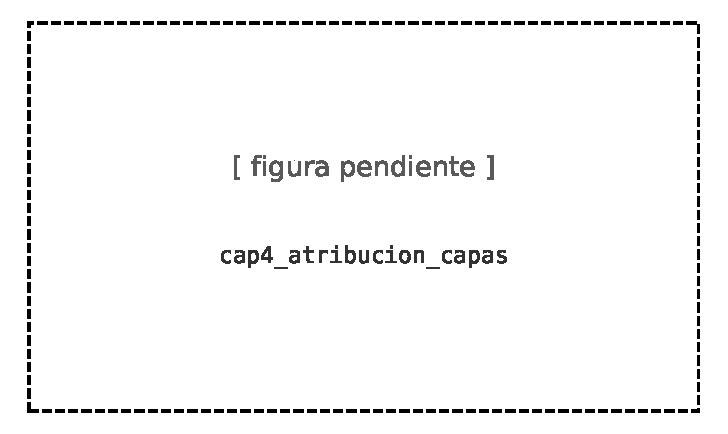
\includegraphics[width=0.9\textwidth]{figuras/cap4_atribucion_capas}
\caption{Reparto de funciones entre las dos capas. A la izquierda, atribución del P\&L de rescate por detector sobre SPY: el canal de régimen (RAM) concentra el $100\,\%$, PSA y GSO aportan cero. A la derecha, evolución diaria del rescate de la regla (riesgo, $\Delta$Sharpe acumulado) frente al del aprendiz (accuracy, aciertos acumulados sobre el agente): cada serie sube por un eje distinto. Fuente: \texttt{spy\_intervention\_anatomy.json}, \texttt{bullbear\_confirmatory.json}.}
\label{fig:mp-capas}
\end{figure}

\subsection{La ley del \emph{leverage}}
\label{sec:mp-mec-ley}

Si el aprendiz rescata la accuracy, queda la pregunta: ¿lo hace por igual en todos los activos, o hay un orden? Lo hay, y lo gobierna una sola propiedad. El rescate del aprendiz en accuracy escala con el \emph{leverage effect} del activo. Medimos el rescate como la mejora de accuracy del mejor aprendiz sobre el agente, $\max(\mathrm{M10},\mathrm{AutoML}) - \mathrm{M5}$, y la naturaleza del activo con la correlación de Black,
\[
  \mathrm{leverage\_corr} = \operatorname{corr}\!\bigl(r_t,\ \mathrm{RV}^{21}_{t+1} - \mathrm{RV}^{21}_t\bigr),
\]
entre el retorno de hoy y el cambio de la volatilidad realizada a veintiún días (Black 1976 \cite{black1976}; Christie 1982 \cite{christie1982}). Es negativa cuando una caída eleva la volatilidad de mañana, la firma del \emph{leverage} estándar.

Las dos magnitudes corren juntas (Tabla~\ref{tab:mp-ley}, Figura~\ref{fig:mp-scatter}). El \emph{leverage} más negativo, más rescate del aprendiz: Pearson $r = -0{,}56$ ($p = 0{,}093$), Spearman $\rho = -0{,}59$ ($p = 0{,}074$) sobre los diez. La correlación es fuerte y la tendencia es significativa al nivel $\alpha = 0{,}10$ que el proyecto fijó de antemano. Nueve de los diez activos la siguen; ROKU es la única excepción, con \emph{leverage} casi nulo y un rescate alto. Partido el panel en dos, los activos de \emph{leverage} fuerte reciben un rescate medio de $0{,}097$ y los de \emph{leverage} débil de $0{,}059$. El mecanismo es el de la Sección~\ref{sec:mp-panel-riesgo}: cuando el régimen es direccional (\emph{leverage} estándar) la regla ya disciplina el riesgo y al aprendiz le queda margen para afinar la dirección; cuando el régimen no informa el signo, el aprendiz rescata por otra vía y la ganancia se estrecha.

Aquí la honestidad manda, y la decimos antes de que la pregunte el tribunal. Con $n = 10$ no afirmamos $p < 0{,}05$ ni robustez \emph{leave-one-out}: el test es menos potente que la correlación es fuerte, y por eso la presentamos como tendencia al $\alpha = 0{,}10$, no como ley exacta. Una segunda cautela es de dirección. La naturaleza del activo ordena el rescate del \emph{aprendiz}, pero no predice el valor de la \emph{regla}: ninguna propiedad de la naturaleza (\texttt{crisis\_mean}, \emph{leverage} o sesgo del agente) correlaciona con el rescate de la regla a ningún nivel razonable (todas con $p > 0{,}14$). El \texttt{crisis\_mean} es descriptivo, no ley. La única ley del rescate es la del \emph{leverage} sobre el aprendiz.

\begin{table}[htbp]
\centering
\caption{Ley del \emph{leverage}: correlación de Black y rescate del aprendiz por activo (panel de diez), ordenados por \emph{leverage} creciente. Rescate ${}= \max(\mathrm{M10},\mathrm{AutoML}) - \mathrm{M5}$ en accuracy. Nueve de los diez siguen la tendencia (a más \emph{leverage} negativo, más rescate); ROKU es la excepción. Sobre los diez: Pearson $r = -0{,}56$ ($p = 0{,}093$), Spearman $\rho = -0{,}59$ ($p = 0{,}074$); tendencia significativa al $\alpha = 0{,}10$ pre-registrado. Fuente: \texttt{leverage\_law\_panel10.json}.}
\label{tab:mp-ley}
\begin{tabular}{lrrl}
\toprule
Activo & \texttt{leverage\_corr} & Rescate aprendiz & \\
\midrule
DIA  & $-0{,}112$ & $0{,}080$ & \\
SPY  & $-0{,}110$ & $0{,}207$ & \\
QQQ  & $-0{,}092$ & $0{,}116$ & \\
XLF  & $-0{,}091$ & $0{,}097$ & \\
XLE  & $-0{,}089$ & $0{,}085$ & \\
XLK  & $-0{,}086$ & $0{,}080$ & \\
MARA & $-0{,}059$ & $0{,}016$ & \\
SMCI & $-0{,}004$ & $0{,}068$ & \\
ROKU & $+0{,}003$ & $0{,}100$ & (excepción) \\
UNG  & $+0{,}041$ & $0{,}008$ & \\
\midrule
\emph{leverage} fuerte (media) & & $0{,}097$ & \\
\emph{leverage} débil (media)  & & $0{,}059$ & \\
\bottomrule
\end{tabular}
\end{table}

\begin{figure}[htbp]
\centering
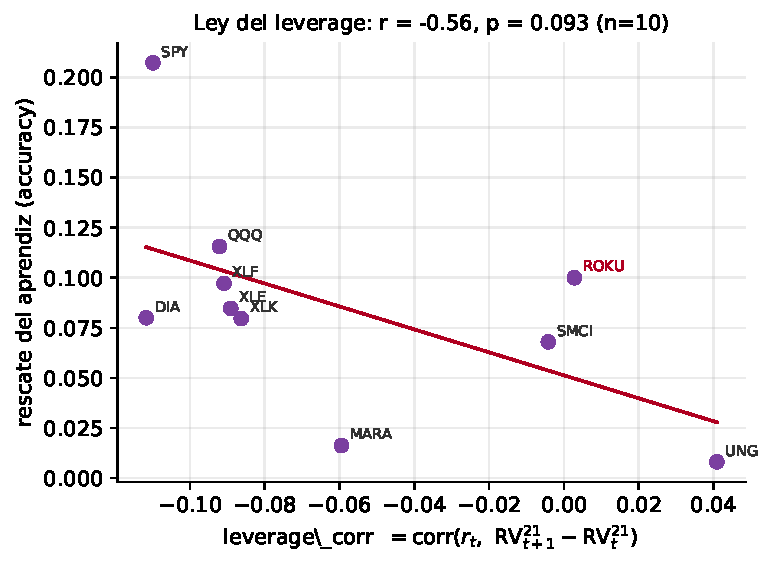
\includegraphics[width=0.85\textwidth]{figuras/cap4_scatter_leverage}
\caption{Rescate del aprendiz en accuracy frente al \emph{leverage} del activo, sobre los diez. Cada punto es un activo; el eje horizontal es la correlación de Black $\operatorname{corr}(r_t,\ \mathrm{RV}^{21}_{t+1}-\mathrm{RV}^{21}_t)$, el vertical el rescate $\max(\mathrm{M10},\mathrm{AutoML}) - \mathrm{M5}$. La recta de regresión baja con el \emph{leverage}: a más \emph{leverage} negativo, más rescate (Pearson $r = -0{,}56$, $p = 0{,}093$; tendencia significativa al $\alpha = 0{,}10$ pre-registrado). Nueve de los diez la siguen; ROKU, señalado, es la excepción. Fuente: \texttt{leverage\_law\_panel10.json}.}
\label{fig:mp-scatter}
\end{figure}

\subsection{Clustering: la naturaleza dibuja los grupos}
\label{sec:mp-clustering}

La ley del \emph{leverage} es una recta. La última pregunta es si esa misma estructura aparece cuando no le decimos al algoritmo qué buscar. La respuesta es que sí: agrupar los diez activos por su naturaleza recupera los mismos bloques que el rescate dibuja, sin ver ni una métrica de rescate. Describimos cada activo por cinco rasgos de naturaleza (\emph{leverage}, retorno medio en Crisis, fracción de días en Crisis, volatilidad OOS y sesgo direccional del agente) y lo agrupamos con cuatro métodos: $k$-medias (MacQueen 1967 \cite{macqueen1967}; Lloyd 1982 \cite{lloyd1982}), enlace de Ward (Ward 1963 \cite{ward1963}), mezcla gaussiana (Dempster \emph{et al.} 1977 \cite{dempster1977}) y clustering espectral (Ng \emph{et al.} 2002 \cite{ng2002spectral}).

Los cuatro coinciden. Con tres grupos, el índice de Rand ajustado entre cualquier par de métodos es $1{,}0$ (Hubert y Arabie 1985 \cite{hubert1985}) y la silueta media es $0{,}55$: una partición unánime y bien separada. Los tres grupos son los de la Tabla~\ref{tab:mp-cluster}, y cada uno trae asociado un canal de rescate distinto:
los índices de \emph{leverage} fuerte (SPY, QQQ, XLF, DIA, XLK, XLE), donde el mejor canal es AutoML;
los de \emph{leverage} invertido (SMCI, UNG), donde el mejor canal es M10;
y los volátiles (ROKU, MARA), donde de nuevo gana AutoML.

El cierre lo da la geometría. Al proyectar la naturaleza de los diez sobre sus dos primeras componentes principales, el primer eje recupera casi exactamente el \emph{leverage}: la correlación entre la primera componente y \texttt{leverage\_corr} es $r = 0{,}84$ (Figura~\ref{fig:mp-pca}). Sin etiquetas de rescate, el clustering ordena los activos por el mismo eje que la ley de la Sección~\ref{sec:mp-mec-ley}. La cadena queda cerrada: la naturaleza del activo define un eje, ese eje es el \emph{leverage}, y el \emph{leverage} ordena qué canal lo rescata. La Figura~\ref{fig:mp-casos} lo aterriza en dos casos trabajados, XLE rescatado por el régimen y MARA por la vía del \emph{leverage} invertido.

Una cautela, la misma del principio. Esto es exploratorio: con diez activos el clustering describe, no confirma. El cluster predice el \emph{tipo} de canal que rescata cada grupo, no el modelo exacto que ganará por activo: qué derivada concreta lidera puede cambiar dentro de un mismo grupo, y eso no es predecible con $n = 10$. La estructura es robusta como dibujo; no la presentamos como regla de asignación.

\begin{table}[htbp]
\centering
\caption{Clustering de la naturaleza de los diez activos (cinco rasgos: \emph{leverage}, retorno medio en Crisis, fracción en Crisis, volatilidad OOS, sesgo del agente). Arriba, calidad por método con $K = 3$: silueta y Rand ajustado frente a $k$-medias. Abajo, perfil de cada cluster (\emph{leverage} medio) y su mejor canal de rescate. Consenso unánime entre los cuatro métodos (Rand $= 1{,}0$). Fuente: \texttt{cluster\_panel10.json}.}
\label{tab:mp-cluster}
\begin{tabular}{lrr}
\toprule
Método ($K=3$) & Silueta & Rand vs $k$-medias \\
\midrule
$k$-medias       & $0{,}55$ & $1{,}0$ \\
Ward             & $0{,}55$ & $1{,}0$ \\
Mezcla gaussiana & $0{,}55$ & $1{,}0$ \\
Espectral        & $0{,}55$ & $1{,}0$ \\
\midrule
\multicolumn{3}{l}{\emph{Perfil de cluster (naturaleza media y mejor canal)}} \\
\midrule
Cluster & \emph{leverage} medio & Mejor canal \\
\midrule
C0 índices (SPY, QQQ, XLF, DIA, XLK, XLE) & $-0{,}097$ & AutoML \\
C1 \emph{leverage} invertido (SMCI, UNG)  & $+0{,}018$ & M10 \\
C2 volátiles (ROKU, MARA)                 & $-0{,}028$ & AutoML \\
\bottomrule
\end{tabular}
\end{table}

\begin{figure}[htbp]
\centering
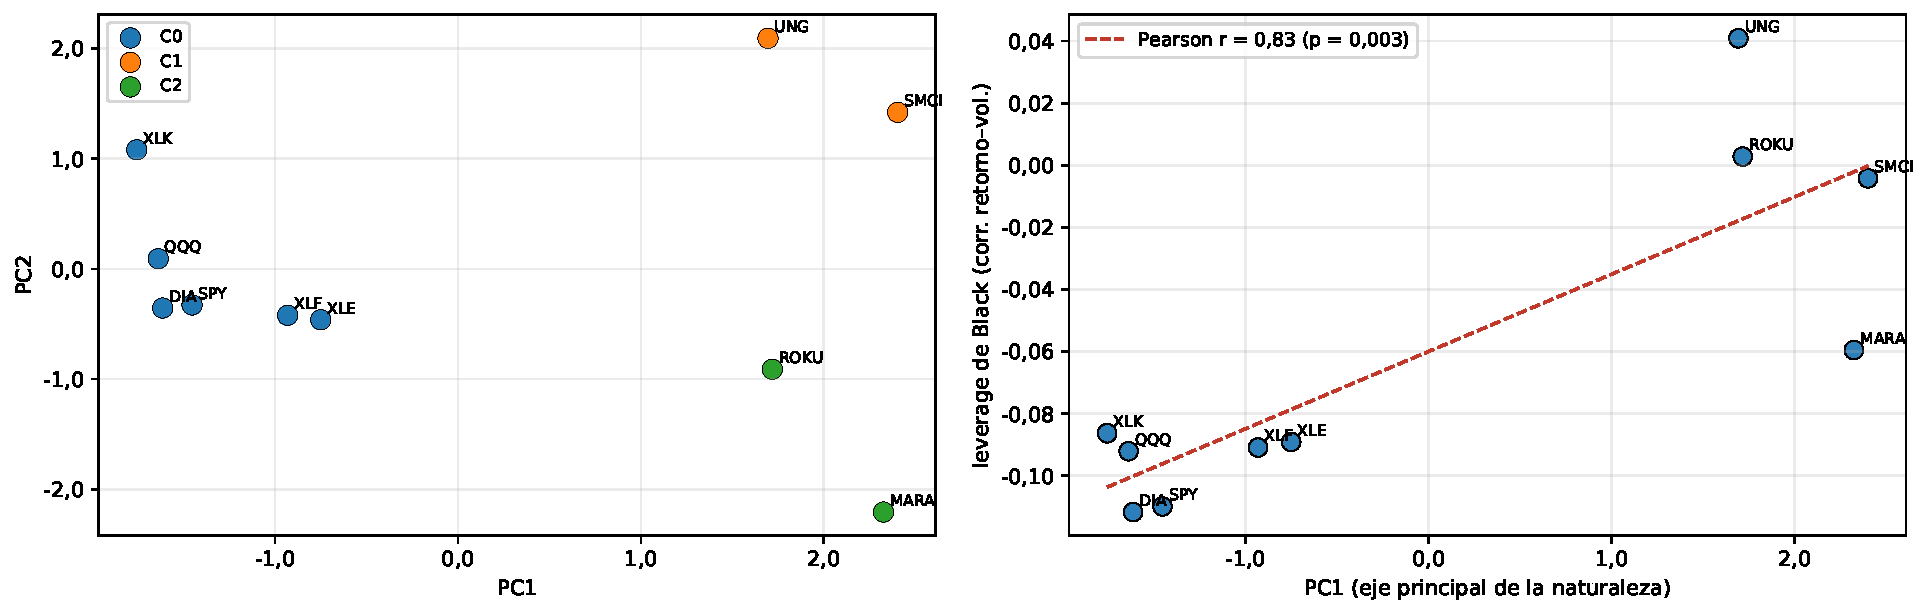
\includegraphics[width=0.85\textwidth]{figuras/cap4_pca_clusters}
\caption{Proyección de la naturaleza de los diez activos sobre sus dos primeras componentes principales. Cada punto es un activo, coloreado por su cluster ($K=3$, partición unánime de los cuatro métodos, Rand $= 1{,}0$). El primer eje recupera el \emph{leverage} ($r = 0{,}84$ entre PC1 y \texttt{leverage\_corr}): el clustering ordena los activos, sin etiquetas de rescate, por el mismo eje que la ley del \emph{leverage}. La leyenda marca el mejor canal de cada grupo (C0/C2 AutoML, C1 M10). Fuente: \texttt{cluster\_panel10.json}, \texttt{mechanism\_panel.json}.}
\label{fig:mp-pca}
\end{figure}

\begin{figure}[htbp]
\centering
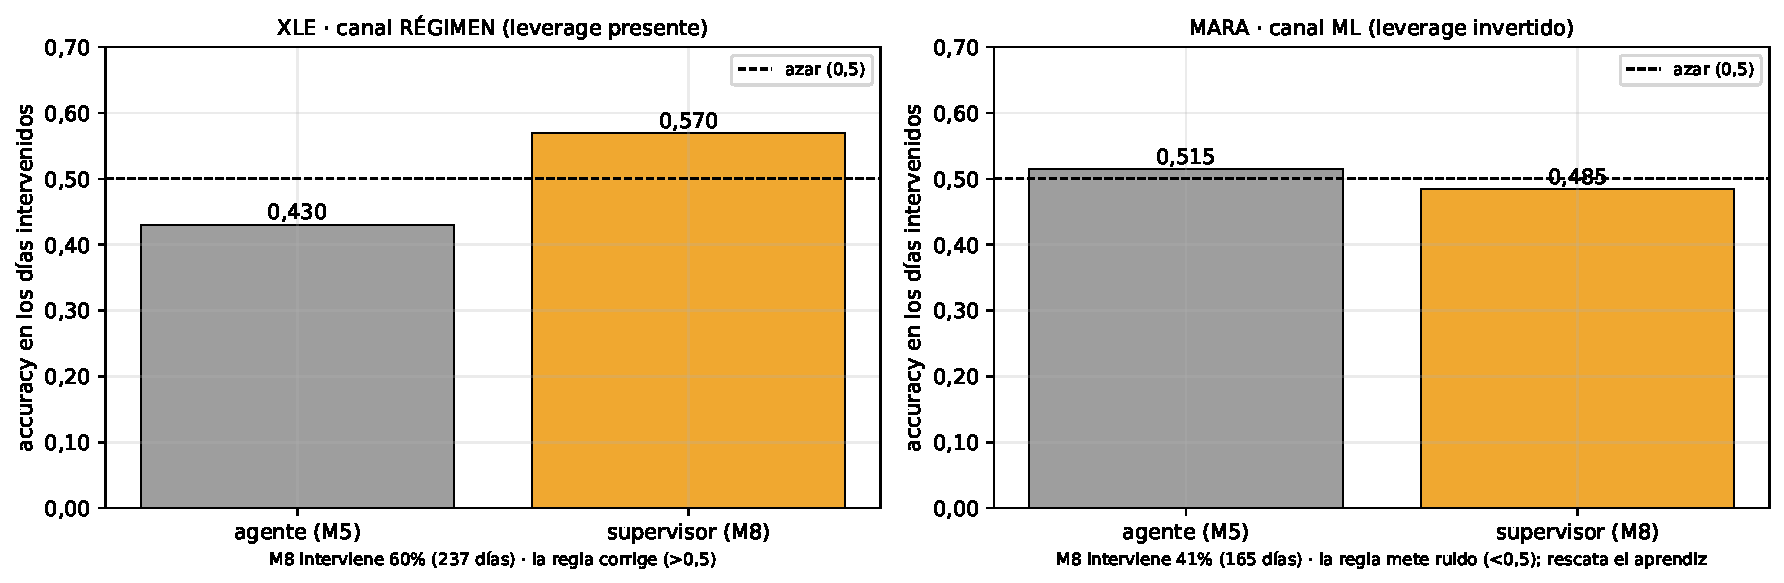
\includegraphics[width=0.9\textwidth]{figuras/cap4_casos}
\caption{Dos casos trabajados, uno por canal. A la izquierda, XLE (\emph{leverage} fuerte): el régimen es direccional y la regla rescata el riesgo del agente. A la derecha, MARA (\emph{leverage} invertido): el régimen no informa el signo y el aprendiz rescata por la vía del sesgo del agente cruzado con el régimen. Cada panel muestra la dirección del agente, la del supervisor que rescata y el régimen vigente. Fuente: \texttt{cluster\_panel10.json}, \texttt{mechanism\_panel.json}.}
\label{fig:mp-casos}
\end{figure}

El reparto de funciones no es casual. La regla protege el riesgo a través del régimen y el aprendiz gana accuracy modelando interacciones no lineales que la regla fija no alcanza; qué canal rescata cada activo lo dicta su naturaleza. El \emph{leverage} ordena el rescate del aprendiz (tendencia significativa al $\alpha = 0{,}10$), el clustering recupera los mismos grupos sin etiquetas (Rand $= 1{,}0$) y su primer eje es de nuevo el \emph{leverage} ($r = 0{,}84$). Cadena cerrada, con la cautela de que sobre diez activos esto es un patrón fuerte, no un teorema. Dónde empieza ese límite, y qué otras afirmaciones no sobreviven a un test, es lo que ordena la Sección~\ref{sec:mp-limites}.
